\documentclass{article}
% For math environments
\usepackage{amsmath, amsfonts}
% For links
\usepackage[colorlinks=true,
    linkcolor = blue,
    urlcolor  = blue,
    citecolor = blue,
    anchorcolor = blue]{hyperref}
% Put space between paragraphs
\usepackage{parskip}
% For figures
\usepackage{tikz}
% Set the margins to not be ridiculous
\usepackage[margin=0.75in]{geometry}
% For multiple columns
\usepackage{multicol}
% For controlling enum/itemize spacing and indentation
\usepackage{enumitem}
% More math symbols
\usepackage{amssymb}
% To change enumerate labels

% For tikz plots
\usepackage{pgfplots}
% This isn't needed but avoids a compiler warning
\pgfplotsset{compat=1.16}

% Allow multi-line equations to be broken across pages
\allowdisplaybreaks

% Use @ as a letter
\makeatletter

% Scale down all tikz coordinates while maintaining font size
\tikzset{every picture/.style={scale=0.45, every picture/.style={}}}


% Macros
% Monospace code
\def\code#1{\texttt{#1}}

% Greek letters
\def\a{\alpha}
\def\b{\beta}
\def\g{\gamma}
\def\d{\delta}
\def\D{\Delta}

% Commands that make life easier
\newcommand\gath[1]{\begin{gather} #1 \end{gather}}
\newcommand\ali[1]{\begin{align} #1 \end{align}}
\newcommand\parens[1]{\left( #1 \right)}
\newcommand\squares[1]{\left[ #1 \right]}
\newcommand\braces[1]{\left\{ #1 \right\}}
\newcommand\angles[1]{\left\langle #1 \right\rangle}
\newcommand\deriv[2]{\frac{d #1}{d #2}}
\newcommand\abs[1]{\left| #1 \right|}
\newcommand\floor[1]{\left\lfloor #1 \right\rfloor}
\DeclareMathOperator{\lcm}{lcm}
\def\non{\nonumber \\}

% Multiline equation space
\def\mlesp{\hspace{1.2cm}}

% For grid diagrams
\newcommand\gridbox[3]{\draw (#1,#2) rectangle (#1+1,#2+1) node[pos=.5] {#3};}
\newcommand\gridboxh[3]{\draw[fill=red!20] (#1,#2) rectangle (#1+1,#2+1) node[pos=.5] {#3};}
\newcommand\gridboxb[3]{\draw[fill=black] (#1,#2) rectangle (#1+1,#2+1) node[pos=.5] {#3};}
\newcommand\gridsym[3]{\node at (#1+0.5,#2+0.5) {$#3$};}
\newcommand\gridblank[2]{\filldraw[draw=gray, color=gray] (#1,#2) rectangle (#1+1,#2+1);}
\newcommand\gridcirc[2]{\draw (#1 + 0.5,#2 + 0.5) circle (0.25);}
\newcommand\cwlab[3]{
  \def\dd{0.15}
  \draw (#1 + \dd - 0.03, #2 + 1 - \dd) node {\scriptsize #3};
}

\def\bbw{3.5}
\def\bbh{2}
\newcommand\bigbox[3]{\draw (#1*\bbw,#2*\bbh) rectangle (#1*\bbw+\bbw,#2*\bbh+\bbh) node[pos=.5] {#3};}
\newcommand\bbtextr[3]{\node[right] at (#1*\bbw,#2*\bbh+0.5*\bbh) {#3};}
\newcommand\bbtextb[3]{\node[align=center] at (#1*\bbw+0.5*\bbw,#2*\bbh+0.5*\bbh) {#3};}

% Box puzzle stock answer
\newcommand\boxans[1]{
  Logic was used to deduce the solution:

  #1

  This was verified using Python as well as shown to be unique with a brute force approach.
}

% Multiple numbers
\newcommand\mn[1]{$#1$'s}

% Commands for problems
\newcommand\problem[4]{
  \section*{#1}

  Question: #3
  
  Answer: #2
  
  Explanation: #4
}
\newcommand\aproblem[4]{\problem{Dec #1}{#2}{#3}{#4}}
\newcommand\cproblem[4]{\problem{Problem #1}{#2}{#3}{#4}}

\def\advent@xxiv@i{
  Eve writes down five different positive integers.
  The sum of her integers is $16$. What is the product of her integers?
}

\def\advent@xxiv@ii{
  $14$ is the smallest even number that cannot be obtained by rolling two $6$-sided dice and finding the product of the numbers rolled.

  What is the smallest even number that cannot be obtained by rolling one hundred $100$-sided dice and finding the product of the numbers rolled?
}

\def\advent@xxiv@iii{
  There are $5$ ways to write $5$ as the sum of positive odd numbers:
  \begin{itemize}
    \item $1 + 1 + 1 + 1 + 1$
    \item $1 + 1 + 3$
    \item $3 + 1 + 1$
    \item $1 + 3 + 1$
    \item $5$
  \end{itemize}

  How many ways are there to write $14$ as the sum of positive odd numbers?
}

\def\advent@xxiv@iv{
  The geometric mean of a set of $n$ numbers is computed by mulitplying all the numbers together, then taking the $n$th root.
  The factors of $9$ are $1$, $3$, and $9$.
  The geometric mean of these factors is
  \gath{
    \sqrt[3]{1 \times 3 \times 9} = \sqrt[3]{27} = 3
  }
  What is the smallest number where the geometric mean of its factors is $13$?
}

\def\advent@xxiv@v{
  The sum of $11$ consecutive integers is $2024$.
  What is the smallest of the $11$ integers?
}

\def\advent@xxiv@vi{Put the digits 1 to 9 (using each digit exactly once) in the boxes so that the sums are correct. The sums should be read left to right and top to bottom ignoring the usual order of operations. For example, 4+3×2 is 14, not 10. Today's number is the product of the numbers in the red boxes.
  The number $n$ has $55$ digits.
  All of its digits are $9$.
  What is the sum of the digits of $n^3$?
}

\def\advent@xxiv@vii{
  What is the obtuse angle in degrees between the minute and hour hands of a clock at 08:22?
}

\def\advent@xxiv@viii{
  It is possible to arrange $4$ points on a plane and draw non-intersecting lines between them to form $3$ non-overlapping triangles:

  \begin{center}
    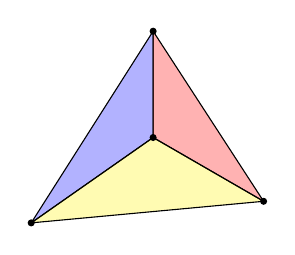
\begin{tikzpicture}
      \def\ds{3}
      \def\pa{(0: 0)}
      \def\pb{(90: \ds)}
      \def\pc{(215: 1.4*\ds)}
      \def\pd{(-30: 1.2*\ds)}

      \def\bcr{3}
      \def\scr{0.55*\bcr}
      \def\sca{34}
      \def\mcr{0.7*\bcr}
      \def\mca{142}
      \def\pr{0.1}

      % Triangles
      \draw[fill=blue,fill opacity=0.3] \pa -- \pb -- \pc -- cycle;
      \draw[fill=red,fill opacity=0.3] \pa -- \pb -- \pd -- cycle;
      \draw[fill=yellow,fill opacity=0.3] \pa -- \pd -- \pc -- cycle;

      % Points
      \fill \pa circle (\pr);
      \fill \pb circle (\pr);
      \fill \pc circle (\pr);
      \fill \pd circle (\pr);
    \end{tikzpicture}
  \end{center}

  It is not possible to make more than $3$ triangles with $4$ points.

  What is the maximum number of non-overlapping triangles that can be made by arranging $290$ points on a plane and drawing non-intersecting lines between them?
}

\def\advent@xxiv@ix{
  Put the digits $1$ to $9$ (using each digit exactly once) in the boxes so that the sums are correct.
  The sums should be read left to right and top to bottom ignoring the usual order of operations.
  For example, $4 + 3 \times 2$ is $14$, not $10$.
  Today's number is the product of the numbers in the red boxes.

  \grid@advent@xxiv@ix{}{}{}{}{}{}{}{}{}
}

\def\advent@xxiv@x{
  A number is a palindrome if it's the same when its digits are written in reverse order.

  What is the sum of all the numbers between $10$ and $100$ that are palindromes?
}

\def\advent@xxiv@xi{
  There are $6$ sets of integers between $1$ and $5$ (inclusive) that contain an odd number of numbers whose median value is $3$:

  \begin{itemize}
    \item $\braces{3}$
    \item $\braces{1,3,4}$
    \item $\braces{2,3,4}$
    \item $\braces{1,3,5}$
    \item $\braces{2,3,5}$
    \item $\braces{1,2,3,4,5}$
  \end{itemize}

  How many sets of integers between $1$ and $11$ (inclusive) are there that contain an odd number of numbers whose median value is $5$?
}

\def\advent@xxiv@xii{
  Holly picks a three-digit number.
  She then makes a two-digit number by removing one of the digits.
  The sum of her two numbers is $309$.
  What was Holly's original three-digit number?
}

\def\advent@xxiv@xiii{
  Today's number is given in this crossnumber.
  No number in the completed grid starts with $0$.

  \begin{multicols}{2}
    \crossnumstd{}{}{}{}{}{}{}{}{}

    \vfill\null
    \columnbreak

    \begin{center}
      \textbf{Across}

      \begin{tabular}{clc}
        \textbf{1} & Today's number.  & (\textbf{3}) \\
        \textbf{4} & Two times 5A.    & (\textbf{3}) \\
        \textbf{5} & A multiple of 1. & (\textbf{3})
      \end{tabular}

      \textbf{Down}

      \begin{tabular}{clc}
        \textbf{1} & Sum of digits is 15. & (\textbf{3}) \\
        \textbf{2} & Sum of digits is 19. & (\textbf{3}) \\
        \textbf{3} & Three times 5A.      & (\textbf{3})
      \end{tabular}
    \end{center}
  \end{multicols}
}

\def\advent@xxiv@xiv{
  $15^3$ is $3375$.
  The last $3$ digits of $15^3$ are $375$.

  What are the last $3$ digits of $15^{1234567890}$?
}

\def\advent@xxiv@xv{
  The number $2268$ is equal to the product of a square number (whose last digit is not $0$) and the same square number with its digits reversed: $36 \times 63$.

  What is the smallest three-digit number that is equal to the product of a square number (whose last digit is not $0$) and the same square number with its digits reversed?
}

\def\advent@xxiv@xvi{
  Put the digits $1$ to $9$ (using each digit exactly once) in the boxes so that the sums are correct.
  The sums should be read left to right and top to bottom ignoring the usual order of operations.
  For example, $4 + 3 \times 2$ is $14$, not $10$.
  Today's number is the product of the numbers in the red boxes.

  \grid@advent@xxiv@xvi{}{}{}{}{}{}{}{}{}
}

\def\advent@xxiv@xvii{
  The number $40$ has $8$ factors: $1$, $2$, $4$, $5$, $8$, $10$, $20$, and $40$.

  How many factors does the number $2^{26} \times 5 \times 7^5 \times 11^2$ have?
}

\def\advent@xxiv@xviii{
  TODO
}

\def\card@xxiv@i{
  What is the largest number you can make by using the digits $1$ to $4$ to make two $2$-digit numbers, then mutiplying the two numbers together?
}

\def\card@xxiv@ii{
  What is the largest number you can make by using the digits $0$ to $9$ to make a $2$-digit number and an $8$-digit number, then mutiplying the two numbers together?
}

\def\card@xxiv@iii{
  The expansion of $(2x+3)^2$ is $4x^2 + 12x + 9$.
  The sum of the coefficients of $4x^2 + 12x + 9$ is $25$.
  What is the sum of the coefficients of the expansion of $(30x + 5)^2$?
}

\def\card@xxiv@iv{
  What is the sum of the coefficients of the expansion of $(2x+1)^{11}$?
}

\def\card@xxiv@v{
  What is the geometric mean of all the factors of $41306329$?
}

\def\card@xxiv@vi{
  What is the largest number for which the geometric mean of all its factors is $92$?
}

\def\card@xxiv@vii{
  What is the sum of all the factors of $7^4$?
}

\def\card@xxiv@viii{
  How many numbers between $1$ and $28988500000$ have an odd number of factors?
}

\def\card@xxiv@ix{
  Eve found the total of the $365$ consecutive integers starting at $500$ and the total of the next $365$ consecutive integers, then subtracted the smaller total from the larger total.
  What was her result?
}

\def\card@xxiv@x{
  Eve found the total of the $n$ consecutive integers starting at a number and the total of the next $n$ consecutive integers, then subtracted the smaller total from the larger total.
  Her result was $22344529$.
  What is the largest possible value of $n$ that she could have used?
}


\begin{document}

\title{Matthew Scroggs 2021 Christmas Card Solutions}
\author{Dan Whitman}
\date{}

\maketitle

Link to the online card: \href{https://www.mscroggs.co.uk/blog/92}{https://www.mscroggs.co.uk/blog/92}

\newcommand\Nodd[1]{N_\mathrm{o}\parens{#1}}

\cproblem{1}{225}{\card@xxi@i}{
  Let $\Nodd{n}$ denote the number of odd integers from $0$ to $n$ inclusive.
  Then clearly
  \ali{
    \Nodd{2n+1} &= \sum_{k=0}n (2k+1) = 2 \sum_{k=0}^n k + \sum_{k=0}^n 1 = 2 \sum_{k=1}^n k + (n+1) \non
    &= 2 \frac{n(n+1)}{2} + n + 1 = n(n+1) + n + 1 = n^2 + 2n + 1 \non
    &= (n+1)^2 \,. \label{eqn:01:Nodd}
  }
  In our case we have $\Nodd{30} = \Nodd{29}$ and $29 = 2 \cdot 14 + 1$ so that our answer is $\Nodd{30} = (14+1)^2 = 225$.
  This was verified in Python with brute force.
}

\cproblem{2}{8031556}{\card@xxi@ii}{
  From the previous problem, $\Nodd{5668} = \Nodd{5667}$ and $5667 = 2 \cdot 2833 + 1$, so that $\Nodd{5668} = (2833+1)^2 = 8031556$ by \eqref{eqn:01:Nodd} above.
  This was also verified in Python with brute force.
}

\def\pval{10000}
\cproblem{3}{445555}{\card@xxi@iii}{
  First, the prime factorization of $\pval$ is
  \gath{
    \pval = 2^4 5^4 \,.
  }
  The only digits that can be formed from products of these primes are $2$, $4 = 2^2$, $5$, and $8 = 2^3$, noting that, in particular, $2 \cdot 5 = 10$ is not a digit or is, for example $5^2 = 25$.
  Hence the answer must have four \mn{5} in it because these cannot be combined to create any other digits.
  The card board provides a hint here as it tells us that the answer has six digits.
  Since there must be four \mn{5}, the $2^4$ factor must comprise two digits.
  The only way to do this is with two \mn{4} since $4 \cdot 4 = 2^4$.
  Therefore the digits must be two $4$'s and four \mn{5}.
  Clearly the smallest number using these is found by just sorting the digits in ascending order, which is $445555$.
  This was verified with Python using brute force.
}

\def\pval{432000}
\cproblem{4}{44555666}{\card@xxi@iv}{
  Similar to the approach of the previous problem, the prime factorization of $\pval$ is
  \gath{
    \pval = 2^7 3^3 5^3 \,.
  }
  Here the only digits that can be formed from these prime factors are clearly $2$, $3$, $4 = 2^2$, $5$, $6=2 \cdot 3$, $8 = 2^3$, and $9 = 3^2$.
  Once again, the answer must contain three \mn{5} since these cannot be combined into other digits.
  Using the card board, the answer must have eight digits.
  So let the following denote the number of each digit in the answer:
  \begin{center}
    \begin{tabular}{c|c}
      Let & Digit \\
      \hline
      $a$ & 9     \\
      $b$ & 8     \\
      $c$ & 6     \\
      $d$ & 4     \\
      $e$ & 3     \\
      $f$ & 2
    \end{tabular}
  \end{center}
  Then, since three of the digits must be \mn{5}, we have
  \gath{
    a + b + c + d + e + f = 8 - 3 = 5 \,. \label{eqn:04:nd}
  }
  of the other digits.
  The digital sum then becomes
  \gath{
    9a + 8b + 5 \cdot 3 + 6c + 4d + 3e + 2f = 41 \non
    9a + 8b + 6c + 4d + 3e + 2f = 26 \label{eqn:04:ds}
  }
  Since \mn{9} use two \mn{3}, \mn{6} use one $3$, and we must have three $3$'s to achieve the digital product, it has to be that
  \gath{
    2a + c + e = 3 \non
    e = 3 - 2a - c \label{eqn:04:3s}
  }
  Similarly, for the digits that use \mn{2}, we must have
  \gath{
    3b + c + 2d + f = 7 \non
    f = 7 - 3b - c - 2d \,. \label{eqn:04:2s}
  }
  Substituting \eqref{eqn:04:3s} and \eqref{eqn:04:2s} into \eqref{eqn:04:nd} results in
  \gath{
    a + b + c + d + (3 - 2a - c) + (7 - 3b - c - 2d) = 5 \non
    -a - 2b - c - d = -5 \non
    a + 2b + c + d = 5 \,. \label{eqn:04:d}
  }
  Similarly, substituting \eqref{eqn:04:3s} and \eqref{eqn:04:2s} into \eqref{eqn:04:ds} gives
  \gath{
    9a + 8b + 6c + 4d + 3(3 - 2a - c) + 2(7 - 3b - c - 2d) = 26 \non
    3a + 2b + c = 3 \,. \label{eqn:04:dio}
  }
  Since everything must be non-negative, \eqref{eqn:04:dio} has three possible solutions:
  \begin{center}
    \begin{tabular}{ccc}
      $a$ & $b$ & $c$ \\
      \hline
      1   & 0   & 0   \\
      0   & 1   & 1   \\
      0   & 0   & 3
    \end{tabular}
  \end{center}
  For the first solution we have $a = 1$ and $b = c = 0$.
  Equation \eqref{eqn:04:d} implies that $d = 4$.
  However, this would mean that the answer contains four \mn{4}, which would require eight \mn{2} since $4^4 = 2^8$.
  As there are only seven \mn{2} available, this solution cannot work.
  In the second solution, $a = 0$ and $b = c = 1$.
  This time \eqref{eqn:04:d} results in $d = 2$ so that \eqref{eqn:04:2s} implies that $f = -1$.
  As this is clearly problematic, this solution does not work either.
  In the third solution, $a = b = 0$ and $c = 3$ so that \eqref{eqn:04:3s} sets $e = 0$, \eqref{eqn:04:d} set $d = 2$, and \eqref{eqn:04:2s} sets $f = 0$.
  None of these are problematic, and they tell us that our solution contains three \mn{6}, two \mn{4}, and no other digits besides the three \mn{5}.
  Once the digits are sorted from smallest to largest to give the smallest integer, our solution becomes $44555666$.
  This was also verified with Python using brute force.
}

\cproblem{5}{333555}{\card@xxi@v}{
  Intuitively and by symmetry, the largest $n$-gon that can fit inside a circle is a regular $n$-gon whose circumradius is the same as the radius of the circle.
  So consider a general regular $n$-gon with circumradius $r$ centered at the origin with one of its vertices aligned at the positive $x$-axis at $p_0 = (r, 0)$.
  Then the angle spanned by each segment is clearly $\phi = 2 \pi / n$, and the next vertex is at the point $p_1 = (r \cos{\phi}, r \sin{\phi})$.
  This is illustrated by the following diagram:
  \begin{center}
    \begin{tikzpicture}
      \def\dr{12}
      \def\ss{0.8}
      \def\pi@x{0.8660254037844387*\dr}
      \def\pi@y{0.5*\dr}
      \def\ar{1}
      \def\cr{0.1}
      \draw (0, 0) -- (\pi@x, \pi@y) node[midway,above]{$r$} -- (\dr, 0) -- cycle node[midway,below]{$r$};
      \draw (\pi@x, 0) -- (\pi@x, \pi@y);
      \draw (\pi@x-\ss, 0) rectangle (\pi@x, \ss);
      \draw (\ar, 0) arc [start angle=0, end angle=30, radius=\ar] node[midway,right,yshift=2]{$\phi$};
      \filldraw[fill=black] (0, 0) circle (\cr);
      \node[left] at (0, 0) {$(0,0)$};
      \filldraw[fill=black] (\pi@x, \pi@y) circle (\cr);
      \node[above] at (\pi@x, \pi@y) {$p_1$};
      \filldraw[fill=black] (\dr, 0) circle (\cr);
      \node[right] at (\dr, 0) {$p_0$};
    \end{tikzpicture}
  \end{center}
  The area of the entire $n$-gon is then $n$ times the area of this segment:
  \gath{
    A = n \frac{1}{2} r (r \sin{\phi}) = \frac{n r^2 \sin{\phi}}{2} \,. \label{eqn:05:A}
  }
  For the dodecagon in our case, clearly $n = 12$ so that $\phi = \sin(2\pi/12) = \sin(\pi/6) = 1/2$ so that
  \gath{
    A = \frac{12 r^2 (1/2)}{2} = 3r^2 \,.
  }
  We are told that the area of the circumscribing circle is
  \gath{
    A_c = 111185 \pi = r^2 \pi \non
    r^2 = 111185 \,.
  }
  Therefore the area of the dodecagon is
  \gath{
    A = 3r^2 = 3 \cdot 111185 = 333555 \,,
  }
  which is of course our answer.
}

\cproblem{6}{345555}{\card@xxi@vi}{
  If we consider a dodecagon with circumradius $r$ centered at the origin that is oriented such that one of the vertices is on the $x$-axis at $(r, 0)$, then clearly each of the vertices will be at an angle of $2 \pi k / 12 = \pi k / 6$ where $0 \leq k \leq 11$.
  In particular, for $k = 6$ there is a vertex at angle $\pi$, which will obviously be at the point $(-r, 0)$.
  If we cut the dodecagon in half along the $x$-axis, the bottom six sides collapse into a single side formed by connecting $(-r, 0)$ to $(r, 0)$ along a segment of the $x$-axis, therefore becoming a heptagon.
  Clearly this is the largest heptagon that will fit in a semicircle of radius $r$ in the upper half-plane.
  Now, we are told that the area of the semicircle is
  \gath{
    A_c = \frac{r^2 \pi}{2} = 115185 \pi \non
    r^2 = 2 \cdot 115185 = 230370 \,.
  }
  Then, from the previous problem, the area of the circumscribed heptagon (which is a semi-dodecagon) is
  \gath{
    A = \frac{3r^2}{2} = \frac{3 \cdot 230370}{2} = 345555 \,,
  }
  which is then our answer.
}

\cproblem{7}{6}{\card@xxi@vii}{
  This problem was solved generally in the 2020, Dec~18 advent problem, in which it was deduced that the number of terms $N(n, k)$ of $(x_1 + \cdots + x_n)^k$ is
  \gath{
    N(n, k) = \binom{n + k - 1}{k}.
  }
  Hence, in our case, we have $N(3, 2) = 6$.
}

\cproblem{8}{847628551}{\card@xxi@viii}{
  From the previous problem, we have that the number of terms is
  \gath{
    N(3, 41172) = \binom{3 + 41172 - 1}{41172} = \binom{41174}{41172} = 847628551 \,.
  }
}

\cproblem{9}{11}{\card@xxi@ix}{
  Here we can utilize the results of the 2016, Dec~14 problem.
  In our case we have $n = 4$ and $m = 5$, which are clearly coprime.
  Therefore, our answer is
  \gath{
    c = nm - n - m = 4 \cdot 5 - 4 - 5 = 11.
  }
}

\cproblem{10}{5555556655}{\card@xxi@x}{
  We again utilize the results of the 2016, Dec~14 problem.
  Here we have $n = 83409$ and $m = 66608$, which were verified to be coprime, so that our answer is
  \gath{
    c = nm - n - m = 83409 \cdot 66608 - 83409 - 66608 = 5555556655
  }
}

\cproblem{11}{81}{\card@xxi@xi}{
  Clearly there are $9$ single-digit numbers that meet this criteria.
  For double-digit numbers, we have $9$ choices for the first digit and then $8$ choices for the second, noting that zero is not included in either.
  Therefore the total number is
  \gath{
    9 + 9 \cdot 8 = 9 \cdot (1 + 8) = 9 \cdot 9 = 81 \,.
  }
  This answer was confirmed with a brute force Python program.
}

\cproblem{12}{986409}{\card@xxi@xii}{
  First we note that clearly any integer with ten digits or more cannot count since there are only $9$ nonzero digits and so one must repeat.
  Using the same approach as in the previous problem, it was reasoned that an integers with $n$ digits have
  \gath{
    N(n) = \prod_{k=0}^{n-1} (9 - k) = \frac{9!}{(9-n)!}
  }
  qualifying numbers.
  Therefore the total number of qualifying integers is
  \ali{
    \sum_{n=1}^9 N(n) &= \sum_{n=1}^9 \frac{9!}{(9-n)!} \non
    &= \frac{9!}{8!} + \frac{9!}{7!} + \frac{9!}{6!} + \frac{9!}{5!} + \frac{9!}{4!} + \frac{9!}{3!} + \frac{9!}{2!} + \frac{9!}{1!} + \frac{9!}{0!} \non
    &= 9 + 9 \cdot 8 + 9 \cdot 8 \cdot 7 + 9 \cdot 8 \cdot 7 \cdot 6 +  \cdot 9 \cdot 8 \cdot 7 \cdot 6 \cdot 5 + 9 \cdot 8 \cdot 7 \cdot 6 \cdot 5 \cdot 4 + 9 \cdot 8 \cdot 7 \cdot 6 \cdot 5 \cdot 4 \cdot 3 \non
    &\mlesp + 9 \cdot 8 \cdot 7 \cdot 6 \cdot 5 \cdot 4 \cdot 3 \cdot 2 + 9 \cdot 8 \cdot 7 \cdot 6 \cdot 5 \cdot 4 \cdot 3 \cdot 2 \cdot 1 \non
    &= 9(1 + 8(1 + 7(1 + 6(1 + 5(1 + 4(1 + 3(1 + 2(1 + 1)))))))) \non
    &= 986409 \,.
  }

  This answer was confirmed with a brute force Python program.
}

\cproblem{13}{4}{\card@xxi@xiii}{
  We know from the 2021, Dec~1 problem that our answer must be $2^2 = 4$.
  This was verified using a brute force Python program.
}

\cproblem{14}{625}{\card@xxi@xiv}{
  We know from the 2021, Dec~1 problem that our answer must be $25^2 = 625$.
  This was verified using a brute force Python program.
}

\end{document}
